\documentclass[11pt,a4paper]{scrartcl}
\usepackage{color}
\usepackage{ifthen}
\usepackage{ifpdf}
\usepackage[headings]{fullpage}
\usepackage{amssymb}
\usepackage{listings}
\lstset{language=Java,breaklines=true}
\ifpdf \usepackage[pdftex, pdfpagemode={UseOutlines},bookmarks,colorlinks,linkcolor={blue},plainpages=false,pdfpagelabels,citecolor={red},breaklinks=true]{hyperref}
  \usepackage[pdftex]{graphicx}
  \pdfcompresslevel=9
  \DeclareGraphicsRule{*}{mps}{*}{}
\else
  \usepackage[dvips]{graphicx}
\fi

\newcommand{\entityintro}[3]{%
  \hbox to \hsize{%
    \vbox{%
      \hbox to .2in{}%
    }%
    {\bf  #1}%
    \dotfill\pageref{#2}%
  }
  \makebox[\hsize]{%
    \parbox{.4in}{}%
    \parbox[l]{5in}{%
      \vspace{1mm}%
      #3%
      \vspace{1mm}%
    }%
  }%
}
   
\newcommand{\refdefined}[1]{
\expandafter\ifx\csname r@#1\endcsname\relax
\relax\else
{$($in \ref{#1}, page \pageref{#1}$)$}\fi}
\date{\today}
\chardef\textbackslash=`\\
\usepackage{pdfpages}
\usepackage[utf8]{inputenc}
\usepackage[T1]{fontenc}
\usepackage[german]{babel}
\usepackage{hyperref}
\hypersetup{
	pdftitle={Pflichtenheft},
	bookmarks=true,
}
\usepackage{csquotes}
\usepackage{pmboxdraw}

\usepackage{fancyhdr}%<-------------to control headers and footers
\usepackage[a4paper,margin=1in,footskip=.25in]{geometry}
\fancyhf{}
\fancyfoot[C]{\thepage} %<----to get page number below text
\pagestyle{fancy} %<-------the page style itself


\usepackage{framed}
\definecolor{shadecolor}{RGB}{220,220,220}
\usepackage{float}


\title{Android GO! App - Testbericht}
\author{Gruppe 3}
\date{10.09.17}

% define custom lists
\usepackage{enumitem}
\usepackage{lipsum}

\def\threedigits#1{%
  \ifnum#1<100 0\fi
  \ifnum#1<10 0\fi
  \number#1}
  
\usepackage{fancyvrb}
\usepackage[dvipsnames]{xcolor}

% redefine \VerbatimInput
\RecustomVerbatimCommand{\VerbatimInput}{VerbatimInput}%
{fontsize=\footnotesize,
 %
 frame=lines,  % top and bottom rule only
 framesep=2em, % separation between frame and text
 rulecolor=\color{Gray},
 %
 commandchars=\|\(\), % escape character and argument delimiters for
                      % commands within the verbatim
 commentchar=*        % comment character
}

\newcommand{\arrow}{\ensuremath{^\rightarrow}}
\DeclareUnicodeCharacter{2192}{\arrow}
%\newcommand{\check}{\ensuremath{^\rightarrow}}
\DeclareUnicodeCharacter{2713}{\checkmark}


\begin{document}

\begin{titlepage}
	\begin{center}
	{\scshape\LARGE \bfseries Testbericht \par}
	\vspace{1cm}
	{\scshape\Large Praktikum der Softwareentwicklung \\ Sommersemester 2017\par}
	\vspace{1.5cm}
	{\huge\bfseries Android GO! App\par}
	\vspace{2cm}
	{\Large\itshape - Gruppe 3 -\par}
	\vfill
	{\bfseries erstellt von:\par}
	Arsenii Dunaev \\
	Florian Kröger \\
	Tina Maria Strößner \\
	Volodymyr Shpylka \\	
	\vfill
	% Bottom of the page
	{\large 10.09.17 \par}	
	\end{center}
\end{titlepage}

\newpage

\tableofcontents

\newpage
\section{Testszenarien und globale Testfälle des Pflichtenhefts}

\subsection{Weggefallene und geänderte Testfälle}\label{weggefallene Testfälle}
Diverse Testszenarien, die im Pflichtenheft definiert wurde, werde nicht getestet, da sie durch Änderungen im Verlauf der Entwicklung nicht mehr zutreffend sind. Dazu gehören:
\begin{itemize}
	\item[/T0020/] Das Ändern des Benutzeraccounts war ein Wunschkriterium und wurde in der Implementierung nicht umgesetzt.
	
	\item[/T0090/] Hier wurde der Ablauf des Anwendungsfalls während der Implementierung verändert: Anstatt dem Benutzer eine Lliste mit Benutzern mit der passenden E-Mail-Adresse zu zeigen, wird direkt dem Benutzer mit der passenden E-Mail-Adresse eine Gruppenanfrage geschickt. Außerdem können weder Mitglieder noch Administratoren die aktuellen Gruppenanfragen in er App sehen, es werden lediglich vollwertige Gruppenmitglieder in der Gruppendetailansicht angezeigt.
	
	\item[/T0130/]\label{130} Das Hinzufügen von Administratoren ist in der Implementierung nicht umgesetzt. Verlässt ein Administrator die Gruppe, wird diese gelöscht. Der erwartete Reaktion des Testfalls ist die Löschung der Gruppe.
	
	\item[/T0140/] Fällt weg, da die Funktion 'Administrator hinzufügen' nicht implementiert wurde.
	
	\item[/T0210/] Fällt weg, da die GO-Ansicht nciht umgesetzt wurde. GOs können in der jeweiligen Gruppendetailansicht angesehen werden.
	
	\item[/T0220/] Das Erfassen des Standorts eines Benutzers und das Übermitteln der aktuellen Standorts-Cluster wird durch zwei verschiedene API-Calls realisiert. Deshalb wird das Testszenario jeweils in zwei separate Testfälle gespalten:
	\begin{enumerate}
		\item[/T0221/] Das Übertragen des Standorts und das korrekte Abspeichern des Standorts in der entspechenden Datenstruktur.\label{221}
		\item[/T0222/] Bei Anfrage das Zurücksenden der korrekt geclusterten Standorte.\label{222}
	\end{enumerate}
	
	\item[/T0230/] Fällt weg, da der Teilnahmestatus nur manuell und nicht automatisch geändert werden kann.
	
	\item[/T0240/] wird nicht separat getestet, sondern duch Verwendung unterschiedlicher in Testszenario /T0220/ abgedeckt.
	
	\item[/T0250/] Fällt weg, da ein GO nur manuell beendet werden kann.
	
	\item[/T0320/] Fällt weg. Benachrichtigungen können dur in den Systemeinstellungen des Endsystems geändert werden.
	
\end{itemize}

\subsection{zusätzliche Tests}
Durch Änderungen der Anwendung während der Entwurfs- und Implementierungsphase, sowie zur Abdeckung von Rand- und Fehlerfällen, werden folgende Testfälle zusätzlich getestet:
\begin{itemize}
	\item[/T0360/]\label{360} Testen der Funktion \textit{registerDevice}, da dies nicht automatisch mit der Anmeldung ausgeführt wird, sondern ein extra API-Call durchgeführt werden muss.
\end{itemize}

\newpage

\section{Unittests}

\subsection{Client}

\subsubsection{Tests für Entity-Klassen}
Die Entity-Klassen bestehen hauptsächlich aus Getter- und Setter-Methoden, die aufgrund ihrer Einfachheit nicht extra getestet werden. Nur die zusätzlichen Methoden (wie z.B. \textit{isAdmin()}-Methode bei der \textit{Group}-Klasse) werden getestet.

\subsection{Tests für Activities}
Die Activity Klassen werden nicht mit Unittests getestet, da die UI beinhalten und sehr schwierig Teil für Teil zu testen sind. Die wurden nach den Google-Guidelines erstellt und während der Implementierung manuell auf dem Gerät getestet und debuggt mit dem Android Studio Debugger.

\subsubsection{Tests für ServerCommands}
Alle ServerCommands werden getestet. Dabei wird jeweils das richtige Parsen der \textit{JSON-Objekte} und der Aufruf der richtigen Methoden der \textit{GroupRepository}-Klasse getestet.

\subsubsection{Tests für Repositories}
\begin{itemize}
	\item[Server Anfragen] Jedes der Repositorien (\textit{UserRepository}, \textit{GroupRepository} und \textit{GoRepository}) besitzt die Methoden, die die Anfragen zum Server gewährleisten. Für jede dieser Methoden wird mithilfe der UnitTests und der Testdaten gecheckt, ob die Anfrage richtig zum Server ankommt und dort richtig bearbeitet wird. Dabei schickt der Server den HTTP status code zurück, der entweder 'OK' (200) oder 'CREATED' (201) lauten soll. Dabei dürfen auch keine Fehler auftreten (z.B. 'Internal Server Error' (500) etc.).
	\item[\textit{on...()}-Methoden] Die \textit{GroupRepository}-Klasse verfügt über mehreren \textit{on[CommandName]()}-Methoden, die durch ServerCommands aufgerufen werden und die die Daten lokal auf dem Endgerät ändern. Die Methode \textit{mockGroupData()} wird benutzt, um die Testdaten zu mocken. Danach werden die \textit{on[CommandName]()}-Methoden mithilfe von UnitTests getestet, dabei wird jedes mal gecheckt, ob die Daten lokal richtig geändert werden.
\end{itemize}

\subsubsection{Tests für Server Kommunikation}
\begin{itemize}
	\item[Upstream] Dieses Package besteht aus dem Serializer (für \textit{JSON-Objekte}) und dem REST API für die Server Anfragen. Diese Klassen werden durch die vorherigen UnitTests abgedeckt.
	\item[Downstream] Die meisten Klassen aus diesem Package implementieren das \textit{FirebaseMessagingService}, dessen Testbarkeit durch die UnitTests sehr niedrig ist. Damit wird dieses Package mithilfe von Systemtests getestet.
\end{itemize}

\subsubsection{Tests für Login}
Die \textit{Login}-Klassen werden auch von Google vorgegeben. Damit wird die Möglichkeit, sich in der App an- und abzumelden, manuell durch die Systemtests getestet.


\newpage

\subsection{Server}

\newpage

\section{Testabdeckung}

\subsection{Client}

\begin{center}
	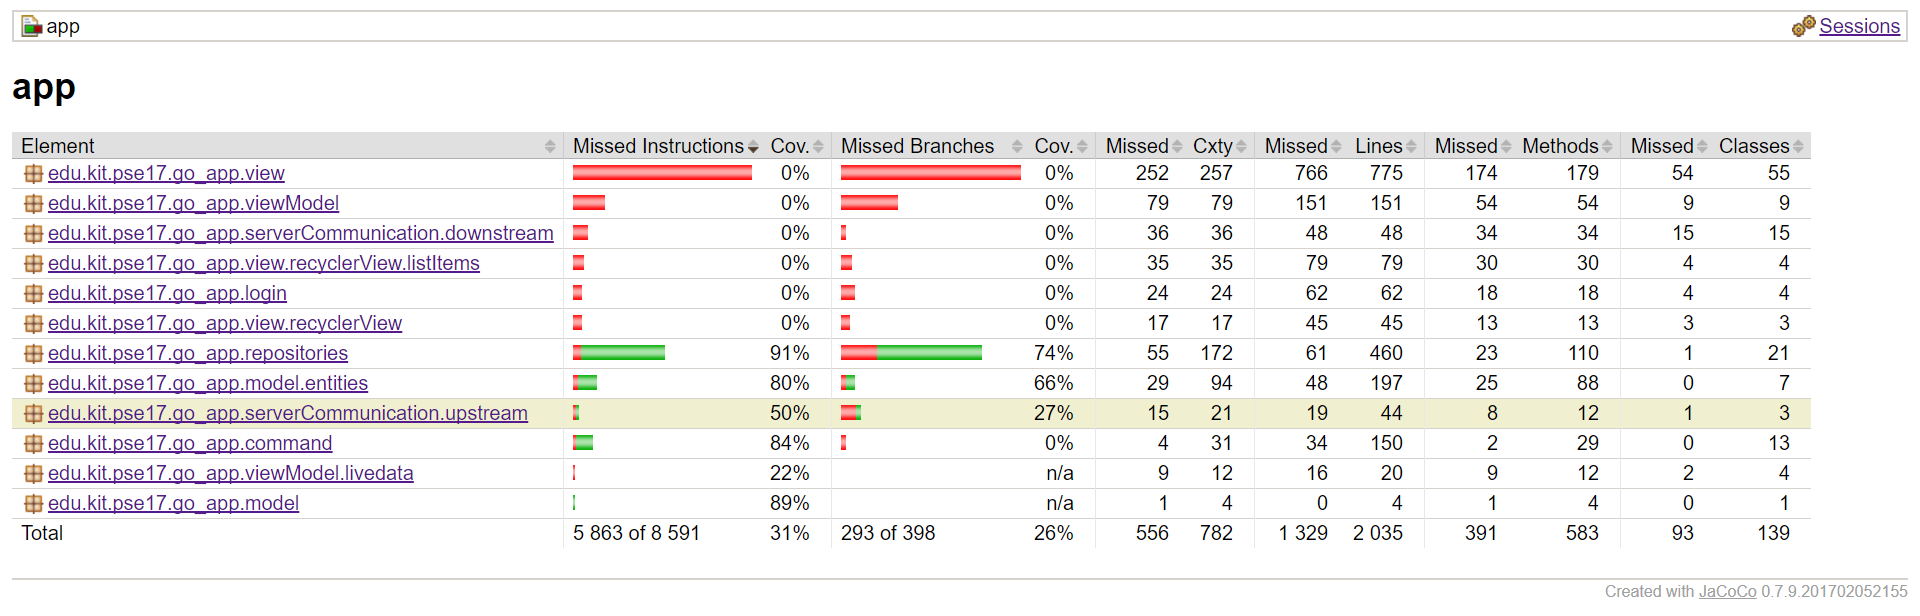
\includegraphics[width=1.0\linewidth]{ClientTestCoverage}
\end{center}

\subsection{Server}

\newpage

\section{Integrationstests}
\subsection{Isolierte Integrationstests der Serveranwendung}\label{ServerIT}
\subsubsection{Erläuterungen zu den Tests}
Tests dieser Art sollen die Funktionsfähigkeit der Serveranwendung testen, ohne dabei die Funktionsfähigkeit der Clients zu berücksichtigen. Dabei wird getestet, ob
\begin{enumerate}
	\item API Calls die richtige Response liefern,
	\item Der Datenbestand in der Datebank nach einem Request wie erwartet manipuliert wurde,
	\item Die Speicherung der Benutzerstandortdaten in den entsprechenden Datenstrukturen korrekt abläuft (nur für Testfall /T0211/),
	\item Benachrichtigungen über Datenänderungen an die richtigen User geschickt wurden,
	\item Der Message Payload der Benachrichtigungen dem richtigen Format und Inhalt entspricht.
\end{enumerate}

Vor einem Testdurchlauf, wird in der Serveranwendung der Testmodus aktiviert. Dadurch werden beim Starten des Programms vordefinierte Testdaten in die GO- und UserLocation-Listen des Location-Services geladen. Darüber hinaus werden wichtige Daten von gespeicherten GOs und UserLocations, sowie versendeten Benachrichtigungen (in der Klasse FcmClient) in .txt-Dateien gespeichert.
Bei der Durchführung eines Testfalls werden folgende Phasen durchlaufen:

\begin{enumerate}
	\item Löschen sämtlicher Daten aus der Datenbank
	\item Ein für den jeweiligen Testfall definierter Anfangsdatenbestand wird in die Datenbank geladen
	\item Es wird ein oder mehrere HTTP-Requests an den Server gestellt. Hierfür wird das Commandline Tool Newman verwendet.
	\item Die Server-Reponse des API Calls wird getestet, auf Korrektheit des HTTP-Statuscodes und des Inhalts des Response-Bodys. Die Testfälle sind in das Newman-Skript integriert und liefern automatisch einen Testbericht, der in einer TestResult-Datei gespeichert wird.
	\item Der Datenbestand der Datenbank nach Beendigung des Newman-Runs wird als .csv-Datei exportiert und mit einer zuvor erstellten .csv-Datei verglichen, die den erwarteten Datenbestand, nach korrekter Ausführung, darstellt. Enthält die .csv ein Datentupel, das nicht erwartet wurde,  wird dieses, zusammen mit der Anzahl der gefundenen Unterschiede, ebenfalss in die TestResult Datei angehängt.
	\item Die aktuellen GOs und die Standortlisten derselben werden in eine Text-Datei exportiert und auf Korrektheit überprüft. Die Ergebnisse werden im Testbericht festgehalten.
	\item Der versendete Message Payload der Observer-Benachrichtigungen wird mit dem erwarteten JSON-String verglichen. Das Ergebnis der Überprüfung wird in der Testresult Datei festgehalten.
	\item Es wird überprüft, ob die versendete Observer-Benachrichtigung an die richtigen Benutzer versendet wurde (keine zusätzlichen Versendungen, keine fehlenden Versendungen).
\end{enumerate}
Einzelne Phasen können ggfs. wegfallen, fallls sie für einen Testfall nicht relevant sind, z.B. wenn es keine Manipulation an der Datenbank gibt oder bei einem API-Call kein Response-Body erwartet wird.\\

Die Ausführung der Testfälle ist mittels eines Shell-Skripts komplett automatisiert. Die benutzten Testdaten und die abgedeckten Testfälle sind dem folgenden Abschnitt zu entnehmen. Dabei sind nicht alle Testfälle des Pflichtenhefts aufgeführt. Auf Testfälle, die gar nicht getestet wurden, wird in Abschnitt \ref{weggefallene Testfälle} eingegangen. Bei weiteren Testfällen, die in diesem Abschnitt nicht auftauchen, kann davon ausgegangen werden, das die getesteten Funktionen keine Beteiligung der Serveranwendung erfordern.\\

Beispielhaft werden hier dast testskript und der testbericht zu Testfall /T0010/ aufgeführt:

\begin{figure}[H]
\VerbatimInput{Server_IntegrationTest/SQL_Skripts/T0010.sh}
\caption{Das Shell-Skript für den Testfall /T0010/}
\end{figure}

\begin{figure}[H]
\VerbatimInput{Server_IntegrationTest/SQL_Skripts/T0010_results.txt}
\caption{Der Testbericht für den Testfall /T0010/}
\end{figure}

Die vollständigen Testberichte der einzelnen Testfälle befinden sich im Anhang.

\newpage

\subsubsection{durchgeführte Tests}
\begin{enumerate}
	\item[\textbf{/T0010/}]
	\textbf{Testfall des Pflichtenhefts: }Der Testfall des Pflichtenhefts beschreibt das erstmalige Einloggen mit einem Google-Account, und damit die Erstellung eines Benutzeraccounts.\\
	\textbf{Anfangsbedingungen: }Die Datenbank enthält noch keine Daten.\\
	\textbf{Umsetzung auf der Serveranwendung: }Der Testfall entspricht dem Aufruf der Methode getData() auf dem Server über die Rest-API, wenn der aufgerufene Benutzeraccount noch nicht in der Datenbank existiert. Es werden drei API-Calls ausgeführt für drei verschiedende Benutzer.\\
	\textbf{Erwartetes Ergebnis: } Der Respose-Body jedes API-Calls besteht aus einer Liste, die eine Dummy-Gruppe mit der Gruppen-ID 1 enthält, da keiner der Benutzer Mitglied in einer Gruppe ist. Nach der Ausführung der API-Calls sind die Benutzer mit den entsprechenden Daten in der Datenbank gespeichert.
	
	\item[\textbf{/T0040/}]
	\textbf{Testfall des Pflichtenhefts: }Ein Benutzer loggt sich in seinem (existierenden) Benutzeraccount ein.\\
	\textbf{Anfangsbedingungen: }Es befinden sich bereits Daten in der Datenbank (3 Benutzer, 1 Gruppe mit 2 Mitgliedern und 1 Gruppenanfrage, 1 Go)\\
	\textbf{Umsetzung auf der Serveranwendung: }Der Tesetfall entspricht dem Aufruf der Methode \textit{getData()} über die Rest-API, wenn der aufgerufene Benutzeraccount bereits existiert. Es wird ein API-Call je angelegtem Benutzer durchgeführt.\\
	\textbf{Erwartetes Ergebnis: }Der Response-Body jedes API-Calls gibt die Struktur der in den Anfangsbedingungen festgelegten Daten wieder. Die Responses sind identisch, da jeder Benutzer mit den gleichen Gruppen assoziiert ist. Es wird keine Manipulation der Daten auf der Datenbank vorgenommen.
	
	\item[\textbf{/T0050/}]
	\textbf{Testfall des Pflichtenhefts: }Ein Benutzer löscht seinen Benutzeraccount\\
	\textbf{Anfangsbedingungen: }Der Benutzer ist mit einem gültigen Account in der Datenbank gespeichert.\\
	\textbf{Umsetzung auf der Serveranwendung: }Die Methode deleteUser() wird aufgerufen. Die Daten des Benutzers, sowie alle Gruppen und Gos, die ihm gehören werden gelöscht.\\
	\textbf{Erwartetes Ergebnis: }Der Testfall-Benutzer ist Adminsitrator einer Gruppe. Es wird erwartet, dass die Gruppe, alle Gruppemmitglieder der Members-Tabelle, alle Requests der Requests-Tabelle, sowie der Eintrag des Benutzers in der Users-Tabelle gelöscht werden.
	
	\item[\textbf{/T0060/}]
	\textbf{Testfall des Pflichtenhefts: }Ein Benutzer erstellt eine neue Gruppe.\\
	\textbf{Anfangsbedingungen:}Der Benutzer ist mit einem gültigen Account in der Datenbank gespeichert.\\
	\textbf{Umsetzung auf der Serveranwendung: }Die Methode createGroup() wird aufgerufen. Im request-Body befindet sich ein gültiger JSON-String, der ein Group-Objekt repräsentiert.\\
	\textbf{Erwartetes Ergebnis: }Der Datenbank wird ein Tupel in der Group-Tabelle hinzugefügt, das dem übergebenen JSON-String entspricht. Darüber hinaus werden entsprechende Einträge in der Members- und Admins-Tabelle hinzugefügt. Der Response-Body enthält die ID unter der die Gruppe in der DB gespeichert ist.
	
	\item[\textbf{/T0070/}]
	\textbf{Testfall des Pflichtenhefts: }Der Name einer Gruppe wird verändert\\
	\textbf{Anfangsbedingungen:}Eine Gruppe ist in der Datenbank gespeichert.\\
	\textbf{Umsetzung auf der Serveranwendung: }Aufruf der Methode editGroup(). Der Request-Body, enthält ein JSON-String, der dem geänderten Group-Objekt entspricht. Dabei sind nur die Attribute ID (zur Identifizierung der Gruppe in der DB), Name und Description relevant. Andere Attribute können auf diese Weise nicht geändert werden. Es wird ein API-Call ausgeführt, der den Namen der Gruppe ändert.\\
	\textbf{Erwartetes Ergebnis: }Der neue Name der Gruppe ist in der Datenbank gespeichert.
	
	\item[\textbf{/T0090/}]
	\textbf{Testfall des Pflichtenhefts: }Der Gruppenadministrator füt ein neues Mitglied hinzu, d.h. er verschickt eine Gruppenanfrage.\\
	\textbf{Anfangsbedingungen:}Eine Gruppe ist in der Datenbank gespeichert und es existieren Benutzer, die nicht mit der Gruppe assoziiert sind.\\
	\textbf{Umsetzung auf der Serveranwendung: }Aufruf der Methode inviteMember() und Übergabe der Email-Adresse des zu hinzufügenden Benutzers. Es werden 2 API-Calls ausgeführt, um 2 Gruppeneinladungen zu verschicken.\\
	\textbf{Erwartetes Ergebnis: }Es werden der Tabelle Requests 2 Tupel hinzugefügt, mit jeweils der ID der Gruppe und der ID des eingeladenen Benutzers.
	
	\item[\textbf{/T0100/}]
	\textbf{Testfall des Pflichtenhefts: }Eine zuvor verschickte Gruppenanfrage wird bestätigt.\\
	\textbf{Anfangsbedingungen:}Es existiert eine Gruppe in der Datenbank und ein Eintrag in der Requests-Tabelle für diese Gruppe und den bestätigenden Benutzer.\\
	\textbf{Umsetzung auf der Serveranwendung: }Aufruf der Methode acceptRequest().\\
	\textbf{Erwartetes Ergebnis: }Der Eintrag der Requests-Tabelle wird entfernt und in die Members-Tabelle eingefügt.
	
	\item[\textbf{/T0110/}]
	\textbf{Testfall des Pflichtenhefts: }Eine zuvor verschickte Gruppenanfrage wird abgelehnt.\\
	\textbf{Anfangsbedingungen:}Es existiert eine Gruppe in der Datenbank und ein Eintrag in der Requests-Tabelle für diese Gruppe und den bestätigenden Benutzer.\\
	\textbf{Umsetzung auf der Serveranwendung: }Aufruf der Methode denyRequest().\\
	\textbf{Erwartetes Ergebnis: }Der Eintrag der Requests-Tabelle wird entfernt.
	
	\item[\textbf{/T0130/}] \label{T130} 
	\textbf{Testfall des Pflichtenhefts: }siehe \ref{130} /T0130/\\
	\textbf{Anfangsbedingungen:}Es existiert eine Gruppe in der Datenbank\\
	\textbf{Umsetzung auf der Serveranwendung: }Aufruf der Methode deleteGroup().\\
	\textbf{Erwartetes Ergebnis: }Die Gruppe, sowie alle Daten, die mit der Gruppe assoziiert (Gos, Members, Admins, Requests), sind werden gelöscht.
	
	\item[\textbf{/T0160/}]
	\textbf{Testfall des Pflichtenhefts: }Ein Mitglied einer Gruppe wird entfernt.\\
	\textbf{Anfangsbedingungen: }Es existiert eine Gruppe in der Datenbank unnd der zu entfernende Benutzer ist nicht der Administrator der Gruppe.\\
	\textbf{Umsetzung auf der Serveranwendung: }Aufruf der Methode removeMember().\\
	\textbf{Erwartetes Ergebnis: }Der Eintrag in der Member-Tabelle wird entfernt. Zusätzlich werden alle Gos des entfernten Benutzers und die damit assoziierten Daten (Going Users, Not Going Users, Gone Users) gelöscht.
	
	\item[\textbf{/T0170/}] wird von Testfall \ref{T130} /T0130/ abgedeckt
	
	\item[\textbf{/T0180/}]
	\textbf{Testfall des Pflichtenhefts: }Erstellen eines GOs\\
	\textbf{Anfangsbedingungen:}Es exisitert eine Gruppe in der Datenbank\\
	\textbf{Umsetzung auf der Serveranwendung: }Aufruf der Methode createGo(). Als Argument wird das im Request-Body als JSON-String übertragene GO-Objekt übergeben.\\
	\textbf{Erwartetes Ergebnis: }Es wird ein Eintrag in der Tabelle GOs erstellt, die dem übergebenen GO-Objekt entspricht. Für den GO-Verantwortlichen wird ein Eintrag in der Tabelle Going-Users erstellt. Für jedes weitere Gruppenmitglied wird ein Eintrag in der Tabelle Not-Going-Users erstellt.
	
	\item[\textbf{/T0200/}]
	\textbf{Testfall des Pflichtenhefts: }Änderung des Teilnahmestatus (im Pflichtenheft von Abgelehnt auf Bestätigt).\\
	\textbf{Anfangsbedingungen:}Es existiert ein Go in der Datenbank.\\
	\textbf{Umsetzung auf der Serveranwendung: }Aufruf der Methode changeStatus(). Der betroffenen Benutzer, sowie der neue Status, werden im Request-Body übergeben. Es werden 3 API-Calls ausgeführt mit jeweils einem Statuswechsel von Going zu Gone, Gone zu Going und Not Going zu Going.\\
	\textbf{Erwartetes Ergebnis: }Der alte Eintrag des Benutzers in den Status-Tabellen (Going-Users, Not-Going-Users, Gone-Users) wird entfernt und ein neuer, entspechend dem neuen Status eingefügt.
	
	\item[\textbf{/T0221/}]
	\textbf{Testfall des Pflichtenhefts: }siehe \ref{221} /T0221/\\
	\textbf{Anfangsbedingungen: }Es befindet sich ein GO in der Datenbank\\
	\textbf{Umsetzung auf der Serveranwendung: }Aufruf der Methode setLocation().\\
	\textbf{Erwartetes Ergebnis: }Speicherung der übermittelten Standortdaten in der UserLocation-Liste des entsprechenden GOs.
	
	\item[\textbf{/T0222/}]
	\textbf{Testfall des Pflichtenhefts: }siehe \ref{222} /T0222/\\
	\textbf{Anfangsbedingungen: }Es befindet sich ein Go in der Datenbank, in der UserLocation-Liste des GOs befinden sich Standortdaten mehrerer Benutzer.\\
	\textbf{Umsetzung auf der Serveranwendung: }Aufruf der Methode \textit{getLocation()}.\\
	\textbf{Erwartetes Ergebnis: }Im Repsose-Body des API-Calls wird eine Lister von Clustern zurückgegeben, die die korrekt geclusterten Standorte repräsentieren.
	
	\item[\textbf{/T0250/}]
	\textbf{Testfall des Pflichtenhefts: }Ein GO wird beendet.\\
	\textbf{Anfangsbedingungen:}Es existiert ein GO in der Datenbank.\\
	\textbf{Umsetzung auf der Serveranwendung: }Die Beendigung eines GOs ist gleichzusetzen mit dem Löschen eines Gos. Es wird die Methode deleteGo() aufgerufen.\\
	\textbf{Erwartetes Ergebnis: }In der Datenbank wird das entsprechende GO gelöscht, sowie alle damit assoziierten Informationen (Einträge in den Status-Tabellen Going-Users, Not-Going-Users und Gone-Users).
	
	\item[\textbf{/T0260/}]
	\textbf{Testfall des Pflichtenhefts: }Die Daten eines GOs werden geändert.\\
	\textbf{Anfangsbedingungen:}Es exisitert ein GO in der Datenbank.\\
	\textbf{Umsetzung auf der Serveranwendung: }Aufruf der Methode editGo(). Die geänderte Gruppe wird dabei als JSON-String im Request-Body übertragen. es wird ein API-Call durchgeführt, der den Namen des GOs ändert.\\
	\textbf{Erwartetes Ergebnis: }Der geänderte Name des GOs wird in der Datenbank gespeichert.
	
	\item[\textbf{/T0360/}]
	\textbf{Testfall des Pflichtenhefts: }siehe \ref{360} /T0360/\\
	\textbf{Anfangsbedingungen:} Es existiert ein Benutzeraccount in der Datenbank.\\
	\textbf{Umsetzung auf der Serveranwendung: }Aufruf der Methode registerDevice(). Es werden drei API-Calls ausgeführt, um allen drei existierenden Benutzern in der Datenbank eine InstanceId zuzuweisen.\\
	\textbf{Erwartetes Ergebnis: }Die InstanceId wird jeweils in dem Tupel des Benutzers in der Datenbank gespeichert.
	
\end{enumerate}

\newpage

\section{Monkey Testing}

Zuerst wurde ein Monkey Test mit 500 zufälligen Events ausgeführt. Danach ein mit 10000 Events, das ist aber viel an einer Stelle geblieben, weil es schon sehr tief in der App war und nicht raus konnte. 1000 random Events geht tief genug in die Activity Hierarchie und bleibt nicht für ewig in einer Activity, wie mit dem Fall mit 10000 Events. Also wurde Monkey Testing mit 1000 zufälligen Events 10 mal ausgeführt. Das hat die App nicht runtergebracht. Das bestätigt die Robustheit der App.

\section{Hallway Usability Test}

\newpage

\section{System Tests}

Während der Implementierung wurde alles manuell getestet und einfach reingeschaut, dass alle funktionale Anforderungen nacheinander korrekt implementiert werden. Für viele Packages der Code sind Unittests und Integrationtests geeignet. Für UI Teil aber nicht so ganz. Deswegen wurde alles manuell auch mit dem Debugger auf einem echten Handy  getestet. Das ist nicht schlimm, da UI sowieso nur View in MVC ist, und wenn es bei der Implementierung richtig angezeigt wird, gibt es meistens sehr wenig Probleme, wenn man nur andere Daten zu UI gibt. Und alle andere Teile von dem Code sind mit automatischen Tests meistens gesichert, also ist die Behebung schnell deswegen.\\

Jede funktionale Anforderung, die alleine für sich getestet werden kann, wurde so während der Implementierungsphase getestet. Die Sachen, wo man zwei Handys braucht (z.B. eine Gruppeneinladung erstellen, oder sehen wie die andere Person den Status ändert) wurden mit zwei echten Handys getestet. Mit getestet ist hier gemeint, dass man auf dem Bildschirm das bekommt, was man erwarten würde. Falls etwas falsch gelaufen ist, dann wurde Code mit dem Debugger durchgegangen und die Fehler meistens schnell lokalisiert, weil Debugger sehr genau ist.\\

Nachdem alle funktionalen Anforderungen für ein Gerät erfüllt wurden, war es noch zu überprüfen, ob zwei Geräte über den Server denselben Zustand besitzen. Basierend auf den funktionalen Anforderungen wurden auch ServerCommands erstellt. Also jetzt sollte einfach systemtisch Command nach Command getestet werden. \\

Man könnte denken, dass so ein Ansatz nicht sehr schnell ist im vergleich zu automatisiserten Tests. Ich habe aber keine zuverlässige Tools gefunden, um System so effizient wie manuell zu testen. Espresso ist meistens die "To go" Tool dafür. Es kommt aber raus, dass es manchmal scheint, undeterministisch zu sein, was sehr frustrierend ist. Es kann auch manche Schaltflächen nicht sehen, d.h. wieder manuelle Beteiligung. Und die Tests laufen dann auch auf dem echten Gerät und brauchen dann ungefähr so viel Zeit, wie der Mensch. Also heute in dem Zustand lohnt sich Espresso für die Systemtests basierend auf UI nicht. Deswegen wurden nur ein Paar geschrieben und gelassen, die wirklich laufen. In unserem Fall lohnt sich der Aufwand aber nicht.\\

\newpage

\section{Bugs}

\begin{enumerate}[label={\textbf{/B\protect\threedigits{\theenumi}0/}}, leftmargin=*]
\item \textbf{FCM-Message nicht an Client gesendet nach dem Löschen einer Gruppe}
	\begin{itemize}
		\item[Symptom]
		Nachdem ein User eine Gruppe gelöscht hat, wird keine Message an die anderen Gruppenmitglieder gesendet, um sie über die Löschung der Gruppe zu informieren. Dies führt zu inkonsistenten Daten auf den verschiedenen Endsystemen.
		\item[Ursache]
		Der GroupRemovedObserver, der für die Versendung der richtigen Message zuständig ist, versucht die zu informierenden Gruppenmitglieder aus der Datenbank zu finden, nachdem die Gruppe in der Datenbank bereits gelöscht wurde. Dies löst eine NullPointerException aus, da auf nicht (mehr) existierende Objekte zugegriffen wird, und das Versenden der Messages wird abgebrochen.
		\item[Behebung]
		Die Receiver-Liste, die der Observer zur Adressierung der Gruppenmitglieder verwendet wird erstellt, \textbf{bevor} die Gruppe aus der Datenbank gelöscht wird. So muss nach der Löschung kein Datenbankzugriff mehr stattfinden, um die Messages korrekt zu senden.
	\end{itemize}

\item \textbf{StackOverflow bei automatisierter JSON Konvertierung}
	\begin{itemize}
		\item[Symptom]
		Das System stürzt ab, sobald ein JSON-String einer Entity-Klasse erstellt werden soll.
		\item[Ursache]
		Durch zyklische Abhängigkeiten (Gruppen entalten GOs, GOs enthalten ein Gruppe) kommt es bei der Konvertierung zu einem StackOverflow.
		\item[Behebung]
		Bevor Entities konvertiert werden, werden die durch die passende \textit{makeJsonable()}-Methode angepasst, sodass sie sicher konvertiert werden können, ohne dass es zu einem StackOVerflow kommt und ohne, dass wichtige Informationen verloren gehen.
	\end{itemize}

\item \textbf{Rückgabe von Null-Werten bei Suche eines Users anhand der Email-Adresse}
	\begin{itemize}
		\item[Symptom] In Anwendungsfällen, in denen ein Benutzer anhand seiner E-Mail-Adresse in der Datenbank gefunden wurde, wird \textit{null} zurückgegeben, wodurch die weitere Abarbeitung des Anwendungsfalls nicht möglich ist.
		\item[Ursache] Die URI, mit der die Anfrage an den Server gestellt wird endet mit der E-Mail-Adresse des Benutzers, woraufhin das '.com' am Ende der E-Mail-Adresse abgeschnitten wird. Durch die fehlende TLD, kann die richtige E-Mail-Adresse in der Datebank nicht identifiziert werden.
		\item[Behebung] Bevor die Anfrage an die Datenbank weitergeleitet wird, wird die Endung '.com' an die gesuchte E-Mail-Adresse angefügt. Da es sich bei den Adressen stets um gmail-Accounts handelt, muss nicht zwischen mehreren TLDs unterschieden werden.
	\end{itemize}
	
\item \textbf{Vertauschung der angezeigten Gruppe, bei Änderung des Gruppennamens}
	\begin{itemize}
		\item[Symptom] Befindet sich ein Benutzer in der Detailansicht einer Gruppe (oder eines GOs) und ändert den Namen derselben (desselben), wird nach Ausführung der Aktion die Detailansicht einer anderen Gruppe (eines anderen GOs) angezeigt.
		\item[Ursache] Die Gruppen und die GOs sind beim Client in einer Liste gespeichert, um sie in der Reihenfolge der Erstellung anzeigen zu können. Wenn ein GO/eine Gruppe geändert wird, wird diese aus der Liste gelöscht und wieder am Ende der Liste hinzugefügt. Da die aktuell angezeigte Gruppe/das GO durch ihren/seinen Index in der \textit{ArrayListe} des \textit{ViewModels} identifiziert wird, wird nach einer Änderung dieser Liste fälschlicherweise die Gruppe/das GO angezeigt, die/das nun diesen Index trägt. Dieser Bug wurde mithilfe der Systemtests gefunden.
		\item[Behebung] Der Bug wird behoben, indem das alte GO/die alte Gruppe durch das neue/die neue auf dem gleichen Platz (mit dem gleichen Index) in der Liste ersetzt wird.
	\end{itemize}
	
\item \textbf{Die neuen Mitglieder der Gruppe nicht zu den alten GOs der Gruppe hinzugefügt}
	\begin{itemize}
		\item[Symptom] Nach der Ergänzung der Gruppe um einen neuen Mitglied wird dieser nicht zu der Liste aller Teilnehmer der alten (schon existirenden) GOs hinzugefügt. Dies führt zu inkonsistenten Daten auf dem Endsystem dieses Benutzers.
		\item[Ursache] Bei der \textit{onMemberAdded()}-Methode der Klasse \textit{GroupRepository}, die die Daten auf den Endsystemen der Benutzer aktualisiert, wurde der Datenbestand der alten GOs der Gruppe nicht geprüft und dabei auch nicht aktualisiert. Dieser Bug wurde mithilfe der Systemtests gefunden.
		\item[Behebung] In der \textit{onMemberAdded()}-Methode werden jetzt alle GOs der Gruppe durchgelaufen und dabei wird der neue Mitglied zu den allen Teilnehmerlisten hinzugefügt.
	\end{itemize}
	
\item \textbf{Die Gruppe auf dem Endsystem des Benutzers, der aus der Gruppe entfernt wird, nicht gelöscht}
	\begin{itemize}
		\item[Symptom] Nach der Entfernung eines Mitglieds der Gruppe wird diese Gruppe auf dem Endsystem dieses Mitglieds weiter angezeigt (statt gelöscht zu werden). Dies führt zum Absturz des Servers, wenn der Benutzer die Gruppe weiter benutzt.
		\item[Ursache] Für den Mitglied der Gruppe, der entfernt wird, wurde dieselbe Verarbeitung gemacht, wie für die anderen Gruppenmitglieder, und zwar nur diese Mitgliedschaft gelöscht (und nicht die Gruppe). Dieser Bug wurde mithilfe der Unittests gefunden.
		\item[Behebung] Falls die Änderung das Endsystem des zu löschenden Mitglieds betrifft, wird bei dem die ganze Gruppe gelöscht.
	\end{itemize}
	
\item \textbf{Aktualisieren der Clusters bei einem falschen GO}
	\begin{itemize}
		\item[Symptom] Wenn der Benutzer aus der \textit{GoDetailActivity} ausgeht, während die Locations ständig in diesem GO aktualisiert werden, und er schaut sich ein anderes GO an, werden die Locations bei einem anderen (falschen) GO geändert.
		\item[Ursache] Bei diesem Vorgehen wurde das GoLiveData beim \textit{GoRepository} mit dem neuen GO, das der Benutzer im GUI gewählt hat, überschrieben. Dabei bekommt die App weiterhin die Locations für das alte GO, die aber im neuen (falschen) GO gespeichert wurden. Dieser Bug wurde mithilfe der Systemtests gefunden.
		\item[Behebung] Die Locations werden jetzt nicht im \textit{GoRepository} aktualisiert, sondern im \textit{GroupRepository} mithilfe der \textit{onLocationsUpdated()}-Methode. Diese Methode bekommt jetzt auch das ID des GOs mit, sodass die Daten konsistent bleiben.
	\end{itemize}

\end{enumerate}

\newpage

\section{Anhang}

\subsection{A. Testberichte zu Abschnitt \ref{ServerIT}}

\subsubsection{Testbericht für Testfall /T0010/}
\VerbatimInput{Server_IntegrationTest/SQL_Skripts/T0010_results.txt}

\newpage
\subsubsection{Testbericht für Testfall /T0040/}
\VerbatimInput{Server_IntegrationTest/SQL_Skripts/T0040_results.txt}

\newpage
\subsubsection{Testbericht für Testfall /T0050/}
\VerbatimInput{Server_IntegrationTest/SQL_Skripts/T0050_results.txt}

\newpage
\subsubsection{Testbericht für Testfall /T0060/}
\VerbatimInput{Server_IntegrationTest/SQL_Skripts/T0060_results.txt}

\newpage
\subsubsection{Testbericht für Testfall /T0070/}
\VerbatimInput{Server_IntegrationTest/SQL_Skripts/T0070_results.txt}

\newpage
\subsubsection{Testbericht für Testfall /T0090/}
\VerbatimInput{Server_IntegrationTest/SQL_Skripts/T0090_results.txt}

\newpage
\subsubsection{Testbericht für Testfall /T0100/}
\VerbatimInput{Server_IntegrationTest/SQL_Skripts/T0100_results.txt}

\newpage
\subsubsection{Testbericht für Testfall /T0100/}
\VerbatimInput{Server_IntegrationTest/SQL_Skripts/T0110_results.txt}

\newpage
\subsubsection{Testbericht für Testfall /T0130/}
\VerbatimInput{Server_IntegrationTest/SQL_Skripts/T0130_results.txt}

\newpage
\subsubsection{Testbericht für Testfall /T0160/}
\VerbatimInput{Server_IntegrationTest/SQL_Skripts/T0160_results.txt}

\newpage
\subsubsection{Testbericht für Testfall /T0170/}
\VerbatimInput{Server_IntegrationTest/SQL_Skripts/T0170_results.txt}

\newpage
\subsubsection{Testbericht für Testfall /T0180/}
\VerbatimInput{Server_IntegrationTest/SQL_Skripts/T0180_results.txt}

\newpage
\subsubsection{Testbericht für Testfall /T0200/}
\VerbatimInput{Server_IntegrationTest/SQL_Skripts/T0200_results.txt}

\newpage
\subsubsection{Testbericht für Testfall /T0250/}
\VerbatimInput{Server_IntegrationTest/SQL_Skripts/T0250_results.txt}

\newpage
\subsubsection{Testbericht für Testfall /T0260/}
\VerbatimInput{Server_IntegrationTest/SQL_Skripts/T0260_results.txt}

\newpage
\subsubsection{Testbericht für Testfall /T0360/}
\VerbatimInput{Server_IntegrationTest/SQL_Skripts/T0360_results.txt}

\end{document}
\grid
